%%%%%%%%%%%%%%%%%%%%%%%%%%%%%%%%%%%%%%%%%%%%%%%%%%%%%%%%%%%%%%%%%%%%%%%%%%%%%%%%

% IEEEconf.cls file must exist in the same directory as the TeX file you want to compile
\documentclass[letterpaper, 10 pt, conference]{IEEEconf}

\title{\LARGE \bf
COMPUTER HISTORY\\
\large The History of the Calculator
}

\author{git-group21\\
\small Ethan Peterson\\
\small Thaddeus Gatlin\\
\small Tharindu Ranasinghe\\
}

% Image/graphics support
\usepackage{graphicx}
\graphicspath{ {./images/} }

% Formatting for lists
\usepackage{enumitem}

% Formatting for media
\usepackage{float}
\restylefloat{table}
\restylefloat{figure}

\begin{document}


\maketitle
\thispagestyle{empty}
\pagestyle{empty}


%%%%%%%%%%%%%%%%%%%%%%%%%%%%%%%%%%%%%%%%%%%%%%%%%%%%%%%%%%%%%%%%%%%%%%%%%%%%%%%%


%%%%%%%%%%%%%%%%%%%%%%%%%%%%%%%%%%%%%%%%%%%%%%%%%%%%%%%%%%%%%%%%%%%%%%%%%%%%%%%%
\section{INTRODUCTION}

We chose to look into the history of calculators. These machines have been around for a very long time. We wanted to see what first drove people to invent these devices and how they were perfected over time into scientific and graphing calculators. 

%%%%%%%%%%%%%%%%%%%%%%%%%%%%%%%%%%%%%%%%%%%%%%%%%%%%%%%%%%%%%%%%%%%%%%%%%%%%%%%%
\section{TIME PERIOD}

Calculators have existed since 2000 BC. The first form of the calculator was called an "Abacus". It was first used by Egyptians and Sumerians. It consisted of a series of rods with beads on them that could be used to perform addition and subtraction faster and with fewer errors. This was done by sliding beads to represent digits within a base ten system. When ten beads were slid up, then one bead was slid up on the next rod and the first ten were reset. This method of performing these calculations can still be used today.
\begin{figure}[h!]
\centering
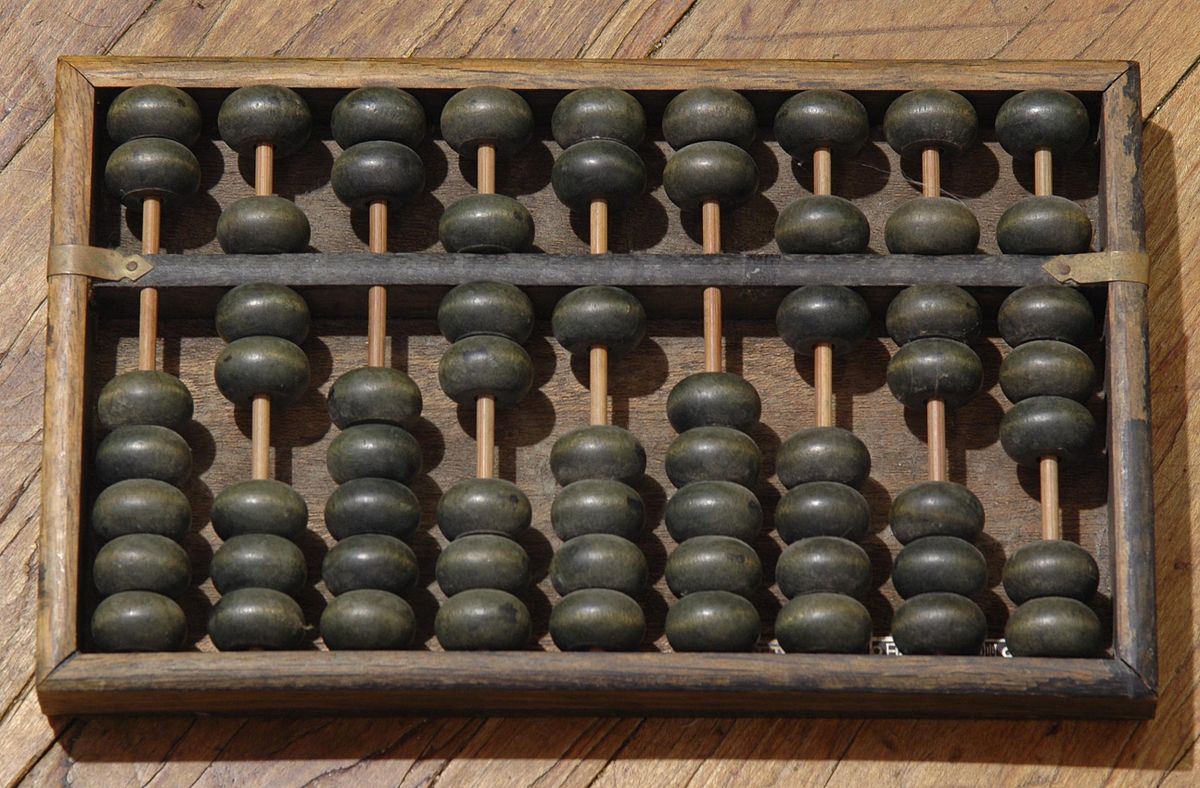
\includegraphics[width=0.45\textwidth]{abacus_pic.jpg}
\caption{Example of a wooden calculator called an "Abacus"}
\label{fig:example}
\end{figure}

%%%%%%%%%%%%%%%%%%%%%%%%%%%%%%%%%%%%%%%%%%%%%%%%%%%%%%%%%%%%%%%%%%%%%%%%%%%%%%%%
\section{COMPUTER HARDWARE}
This method of calculation used in 2000 BC evolved over time
to more intricate machines. The first mechanical calculator
appeared in 1642. It was created by a french mathematician
named Blaise Pascal. It was a machine that used geared wheels
and could add and subtract, it could also divide and multiply
by repetition. 
The first commercially available mechanical calculator was
created in 1851. Calculators improved again in 1930 when they
were used to calculate the trigonometry required to drop bombs
more accurately. These devices were pushed further when they
needed to crack encoded messages as part of their war efforts.

\begin{figure}[h!]
\centering
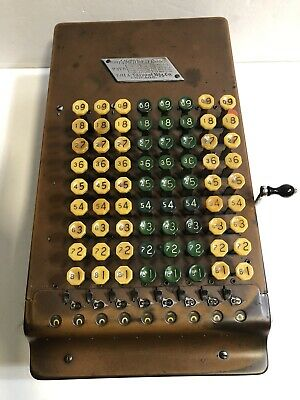
\includegraphics[width=0.25\textwidth]{mechanical_calculator.jpg}
\caption{Example of a mechanical calculator}
\label{fig:example}
\end{figure}

The first electronic calculator was created in 1961 and it was
created for business purposes. It used vacuum and cold cathode
counting tubes to accurately count numbers for office firms.
The introduction of electronic calculators to the workplace
sped up business and helped keep errors down.

\begin{figure}[h!]
\centering
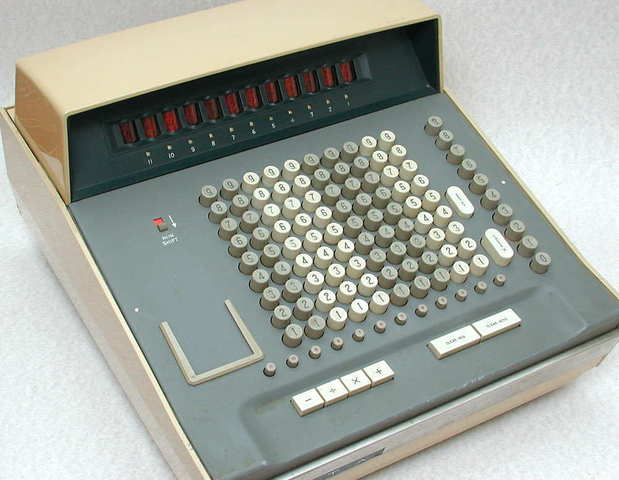
\includegraphics[width=0.25\textwidth]{computer-history.tex/images/office_calculator.jpg}
\caption{First business electronic calculator}
\label{fig:example}
\end{figure}

The next time that calculators had a big leap forward was in 1967 when Texas Instruments released a new innovative design for an electronic calculator that could fit in your hand. This was a massive innovation because before 1967 the smallest calculators were the size of a car battery, but with the invention of the handheld calculator it could be used by everyone.

\begin{figure}[h!]
\centering
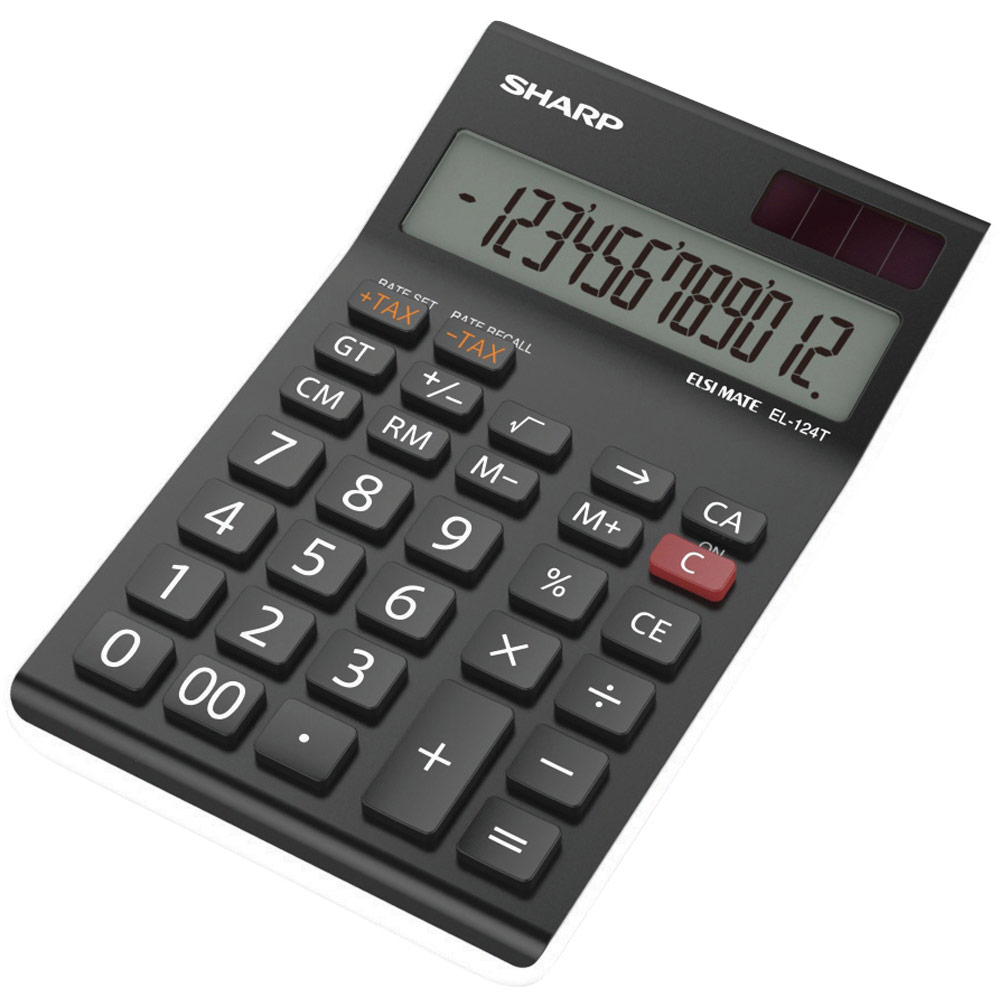
\includegraphics[width=0.25\textwidth]{computer-history.tex/images/calulator_pic.jpg}
\caption{A 20th century calculator}
\label{fig:example}
\end{figure}


\section{COMPUTER SOFTWARE}

Early calculators didn't use software. The first model of the calculator that used software was called "Colossus". It was first utilized in World War II for code breaking. They used a series of algorithms which were then used based on a series of switches when a calculation needed to be done.
\section{CONCLUSION}

Calculators have made everyone's lives easier, especially when being in the world of mathematics. For centuries, they have helped people solve complex problems in an instant. 

\section*{REFERENCES}
\begin{enumerate}[label={[\arabic*]}]
\item Nick Valentine, (March 11, 2019),
''The History Of The Calculator,'' https://www.thecalculatorsite.com/articles/units/history-of-the-calculator.php 
\end{enumerate}

\end{document}

